\documentclass[
  bibliography=totoc,     % Literatur im Inhaltsverzeichnis
  captions=tableheading,  % Tabellenüberschriften
  titlepage=firstiscover, % Titelseite ist Deckblatt
  parskip=half,           % Absätze haben kleinen Abstand und werden nicht eingerückt
  ngerman                 % richtige Übersetzungen (vor Allem für siunitx)
]{scrartcl}

% Pfade sind relativ zum Makefile der Versuche
% Paket float verbessern
\usepackage{scrhack}

% Warnung, falls nochmal kompiliert werden muss
\usepackage[aux]{rerunfilecheck}

% unverzichtbare Mathe-Befehle
\usepackage{amsmath}
% viele Mathe-Symbole
\usepackage{amssymb}
% Erweiterungen für amsmath
\usepackage{mathtools}

% Fonteinstellungen
\usepackage{fontspec}
% Latin Modern Fonts werden automatisch geladen
% Alternativ zum Beispiel:
%\setromanfont{Libertinus Serif}
%\setsansfont{Libertinus Sans}
%\setmonofont{Libertinus Mono}

% Wenn man andere Schriftarten gesetzt hat,
% sollte man das Seiten-Layout neu berechnen lassen
\recalctypearea{}

% deutsche Spracheinstellungen
\usepackage[ngerman]{babel}


\usepackage[
  math-style=ISO,    % ┐
  bold-style=ISO,    % │
  sans-style=italic, % │ ISO-Standard folgen
  nabla=upright,     % │
  partial=upright,   % ┘
  warnings-off={           % ┐
    mathtools-colon,       % │ unnötige Warnungen ausschalten
    mathtools-overbracket, % │
  },                       % ┘
]{unicode-math}

% traditionelle Fonts für Mathematik
\setmathfont{Latin Modern Math}
% Alternativ zum Beispiel:
%\setmathfont{Libertinus Math}

\setmathfont{XITS Math}[range={scr, bfscr}]
\setmathfont{XITS Math}[range={cal, bfcal}, StylisticSet=1]

% Zahlen und Einheiten
\usepackage[
  locale=DE,                   % deutsche Einstellungen
  separate-uncertainty=true,   % immer Unsicherheit mit \pm
  per-mode=symbol-or-fraction, % / in inline math, fraction in display math
]{siunitx}

% chemische Formeln
\usepackage[
  version=4,
  math-greek=default, % ┐ mit unicode-math zusammenarbeiten
  text-greek=default, % ┘
]{mhchem}

% richtige Anführungszeichen
\usepackage[autostyle]{csquotes}

% schöne Brüche im Text
\usepackage{xfrac}

% Standardplatzierung für Floats einstellen
\usepackage{float}
\floatplacement{figure}{htbp}
\floatplacement{table}{htbp}

% Floats innerhalb einer Section halten
\usepackage[
  section % Floats innerhalb der Section halten
]{placeins}

% Seite drehen für breite Tabellen: landscape Umgebung
\usepackage{pdflscape}

% Captions schöner machen.
\usepackage[
  labelfont=bf,        % Tabelle x: Abbildung y: ist jetzt fett
  font=small,          % Schrift etwas kleiner als Dokument
  width=0.9\textwidth, % maximale Breite einer Caption schmaler
]{caption}
% subfigure, subtable, subref
\usepackage{subcaption}

% Grafiken können eingebunden werden
\usepackage{graphicx}

% schöne Tabellen
\usepackage{booktabs}

% Verbesserungen am Schriftbild
\usepackage{microtype}

% Literaturverzeichnis
\usepackage[
  backend=biber,
  natbib=true,     % |
  style=numeric,   % |> ändert die Nummerierung und Sortierung des Literaturverzeichnisses
  sorting=none     % |
]{biblatex}

% Hyperlinks im Dokument
\usepackage[
  german,
  unicode,        % Unicode in PDF-Attributen erlauben
  pdfusetitle,    % Titel, Autoren und Datum als PDF-Attribute
  pdfcreator={},  % ┐ PDF-Attribute säubern
  pdfproducer={}, % ┘
]{hyperref}
% erweiterte Bookmarks im PDF
\usepackage{bookmark}

% Trennung von Wörtern mit Strichen
\usepackage[shortcuts]{extdash}


%--------------------------------------------------------------------------------
% Ab hier optionale Packages, die nicht in der Toolbox-Workshop Vorlage sind.
%--------------------------------------------------------------------------------

% Anpassbare Enumerates/Itemizes
%\usepackage{enumitem}

% Tabellen mit einer Zelle über mehrere Reihen
%\usepackage{multirow}

% Tabellen aus .csv Dateien
%\usepackage{csvsimple}

% Floats innerhalb einer Subsection halten: 
% Hierfür muss in Zeile 78 das below, gelöscht werden
\makeatletter
\AtBeginDocument{%
 \expandafter\renewcommand\expandafter\subsection\expandafter{%
   \expandafter\@fb@secFB\subsection
 }%
}
\makeatother

% um "Overfull \hbox" zu debuggen
%\usepackage{lua-visual-debug}         % alle Latex-Pakete mit Einstellungen
% Differential
\NewDocumentCommand \dif{m} 
{
  \mathinner{\symup{d} #1}
}

% Tabellen Header mit Variable und Einheit
\NewDocumentCommand \tableSI{m m} 
{
  $#1 \:/\: \si{#2}$
}  % Eigene LaTeX-Commands
\author{%
  Nico Guth\\%
  \href{mailto:nico.guth@tu-dortmund.de}{nico.guth@tu-dortmund.de}%
  \and%
  David Venker\\%
  \href{mailto:david.venker@tu-dortmund.de}{david.venker@tu-dortmund.de}%
}
\publishers{TU Dortmund – Fakultät Physik}          % Authoren-Informationen für die Titelseite

% Biblatex Quellen
\addbibresource{../default/bib/lit.bib}
\addbibresource{../default/bib/programme.bib}

\usepackage{minted}

\addbibresource{latex/lit.bib}

\subject{V44}  % Versuchsnummer
\title{Röntgenreflektometrie} % Versuchstitel
\date{%
  Durchführung: 07.06.2021
  \hspace{3em}
  Abgabe: DATUM
}

\begin{document}

\maketitle
\thispagestyle{empty}
\tableofcontents
\newpage

\section{Goals of this Experiment}
\label{sec:Goals}

This experiment should be seen as an introduction to diode laser physics.

A spectroscopy of rubidium will be performed with a diode laser operating in the infrared region using an optical grating.
\section{Theorie}
\label{sec:Theorie}

Die gepulste Kernspinresonanz (bzw. NMR für \enquote{nuclear magnetic resonance}) nutzt, dass Atomkerne mit einem nicht verschwindenden Kernspin an äußere Magnetfelder koppeln.
Diese Wechselwirkung erzeugt eine makroskopische Magnetisierung des Materials und eine Änderung dieser Magnetisierung kann mit einer Spule gemessen werden.
Dadurch können verschiedene Eigenschaften der Probe gemessen werden ohne der Probe Schaden zuzufügen.

Die gepulste Kernspinresonanz wird heutzutage in vielen Bereichen verwendet und 
ist besonders in der Medizin mittels der Magnetresonanztomographie (bzw. MRT) von großer Bedeutung.

\subsection{Magnetisierung in einem konstanten, homogenen Magnetfeld}
\label{ssec:Magnetisierung_konstant}

Ein äußeres homogenes Magnetfeld $B$ führt bei Atomen und auch deren Kernspins zum sogenannten Zeeman-Effekt.
Dabei werden die sonst in der magnetischen Quantenzahl $m$ entarteten Energieniveaus aufgespaltet 
mit einem Energieabstand von
\begin{equation}
    \Delta E = \gamma \hbar B \, .
\end{equation}
Hier ist $\gamma$ der gyromagnetische Faktor und $\hbar$ das Reduzierte Plancksche Wirkungsquantum.
Wir beschränken uns hier auf die Betrachtung von Kernspins von $m=\pm 1/2$, also z.B. Protonen bzw. Wasserstoffkerne.

Der Kernspin kann klassisch auch als ein Drehimpuls $\vec{J}$ angesehen werden, der ein magnetisches Moment $\vec{\mu} = \gamma \vec{J}$ erzeugt.

Ein Magnetfeld $\vec{B}$ führt nun zu einem Drehmoment auf dem Kernspin von
\begin{equation}
    \vec{D} = \frac{\symup{d} \vec{J}}{\symup{d} t} = \vec{\mu} \times \vec{B} \, .
\end{equation}
Wenn nun das Magnetfeld homogen und konstant mit Stärke $B_0$ in $z$-Richtung zeigt, 
dann präzediert $\vec{\mu}$ um die $z$-Achse mit der sogenannten Larmorfrequenz $\nu_0$.
Diese Frequenz kann über
\begin{equation}
    \nu_0 = \frac{\omega_0}{2 \pi} = - \frac{\gamma B_0}{2 \pi}
    \label{eq:Larmorfrequenz}
\end{equation}
berechnet werden, wobei $\omega_0$ die Kreislarmorfrequenz ist.

Im thermischen Gleichgewicht stellt sich eine makroskopische Magnetisierung $\vec{M} = \sum_i <\vec{\mu}_i>$ in die $z$-Richung ein.

\subsection{Magnetisierung in einem magnetischen Wechselfeld}
\label{ssec:Magnetisierung_wechsel}

Wenn nun zusätzlich zum konstanten und homogenen Magnetfeld $\vec{B}_0 = (0,0,B_0)^T$ ein magnetische Wechselfeld
$\vec{B}_1 = (B_1 \sin(\omega_\text{WF} t),B_1 \cos(\omega_\text{WF} t),0)^T$ geschaltet wird, verändert sich die Magnetisierung der Probe.
Es sollte $\Delta \omega = \omega_0 - \omega_\text{WF} \approx 0$ gewählt werden.
Dieses Wechselfeld entspricht im Experiment dem gepulsten Wechselfeld, das durch eine Spule um die Probe erzeugt wird.

Es ist sinnvoll in ein rotierendes Koordinatensystem überzugehen, das eine Frequenz $\omega_\text{RKS} = \omega_\text{WF}$ besitzt.
Hier ergibt sich das gesammte bzw. effektive Magnetfeld zu
\begin{equation}
    \vec{B}_\text{eff} = (0, B_1, B_0 + \frac{\omega_\text{WF}}{\gamma})^T
\end{equation}
und in diesem Koordinatensystem präzediert ein magnetisches Moment mit 
\begin{equation}
    \vec{\omega}_\text{eff} = (0, \omega_\text{WF}, \Delta \omega)^T \, .
\end{equation}

Für die Magnetisierung entsteht so die Bewegungsgleichung 
\begin{equation}
    \left( \frac{\symup{d} \vec{M}}{\symup{d} t} \right)_\text{RKS} = \left( \vec{\omega}_\text{eff} \times \vec{M} \right) \, .
    \label{eq:M_beweg}
\end{equation}
Unter der Vorraussetzung $\Delta \omega = 0$ präzediert also die Magnetisierung im rotierenden Koordinatensystem um die $y$-Achse mit $\omega_1 = - \gamma B_1$.
Auch die einzelnen Kernspin-Momente $\vec{\mu}_i$ präzedieren um die $y$-Achse.

Diese Präzession kann genutzt werden, um mit einem gepulsten, also nur kurz eingeschaltetem Wechselfeld die Magnetisierung aus dem thermischen Gleichgewicht auszulenken.
Ein Puls der Länge $t_\text{P}$ dreht die Magnetisierung um den Winkel
\begin{equation}
    \alpha = \gamma B_1 t_\text{P}
\end{equation}
und die Pulse werden typischerweise nach diesem Winkel benannt.
So dreht ein $\SI{90}{\degree}_y$-Puls die Magnetisierung um $\SI{90}{\degree}$ um die $y$-Achse des rotierenden Koordinatensystems. 
Analog ist z.B. auch ein $\SI{180}{\degree}_y$-Puls definiert.

\subsection{Relaxationseffekte}
\label{ssec:Relaxationseffekte}

Sobald die Magnetisierung aus der thermischen Gleichgewichtslage ausgelenkt wurde und das Wechselfeld abgeschaltet wurde,
fängt die Probe an wieder in ein thermisches Gleichgewicht zu relaxieren.
Unter der Vorraussetzung $\Delta \omega = 0$ lassen sich aus \autoref{eq:M_beweg} die sogenannten Bloch-Gleichungen 
\begin{align}
    \left( \frac{\symup{d} M_x}{\symup{d} t} \right)_\text{RKS} &= \left( -\frac{M_x}{T_2} \right)
    \label{eq:Bloch_x} \\
    \left( \frac{\symup{d} M_y}{\symup{d} t} \right)_\text{RKS} &= \left( -\frac{M_y}{T_2} \right)
    \label{eq:Bloch_y} \\
    \left( \frac{\symup{d} M_z}{\symup{d} t} \right)_\text{RKS} &= \left( -\frac{M_z - M_\infty}{T_2} \right)
    \label{eq:Bloch_z} 
\end{align}
ableiten, die beschreiben wie die Probe relaxiert.
$M_\infty$ ist hier die Magnetisierung im thermischen Gleichgewicht und $T_1$ und $T_2$ sind Zeitkonstanten, die im Folgenden erläutert werden.

\subsubsection{Spin-Gitter-Relaxation}
\label{sssec:Spin-Gitter-Relaxation}

Ohne äußeres Magnetfeld sind die Kernspin-Momente willkürlich ausgerichtet.
Mit einem äußeren Magnetfeld ist die potentielle Energie eines magnetischen Dipols
\begin{equation}
    E_\text{pot} = - \vec{\mu} \cdot \vec{B}
\end{equation}
und wird somit minimal wenn der Dipol entlang der Feldlinien ausgerichtet ist.
Dies führt nun bei unserer Probe im Magnetfeld $B_0$ entlang der $z$-Achse aufgrund von thermischen Schwankungen dazu, 
dass die Kernspin-Momente im Mittel in eine Magnetisierung entlang der $z$-Achse relaxieren.
Dabei wird von den Kernspin-Momenten die potentielle Energie in Gitter-Schwingungen umgewandelt.
Dieser Vorgang heißt Spin-Gitter-Relaxation und wird durch die Zeitkonstante $T_1$ charakterisiert.

\subsubsection{Spin-Spin-Relaxation}
\label{sssec:Spin-Spin-Relaxation}

Wenn z.B. durch einen $\SI{90}{\degree}_y$-Puls eine Netto Magnetisierung in der $xy$-Ebene entsteht, wird diese mit der Zeit zerfallen.
Dies geschieht weil das äußere Magnetfeld Fluktuationen aufweist, die Spins sich gegenseitig beeinflussen und somit die Phasen des präzidierenden Kernspin-Momenten auseinander laufen.
Dieser Vorgang heißt Spin-Spin-Releaxation und wird durch die Zeitkonstante $T_2$ charakterisiert.

\subsubsection{Feldinhomogenitäten}
\label{sssec:Feldinhomogenitäten}

Da es in der Realität nicht möglich ist ein konstantes und homogenes Magnetfeld ohne Ingomogenitäten zu erzeugen,
sind diese Feldinhomogenitäten mit zu betrachten.
Aufgrund von \autoref{eq:Larmorfrequenz} und den örtlich unterschiedlichen Feldstärken besitzen nicht alle Kernspins die gleiche Larmorfrequenz.
Dies führt dazu, dass die Kernspin-Momente wie bei der Spin-Spin-Relaxation ihre Phasenbeziehung verlieren.
Der Unterschied liegt jedoch darin, dass diese durch Feldinhomogenitäten verursachte dephasierung reversibel ist, da die Kernspins näherungsweise ihren Ort im Magnetfeld nicht velassen.

\subsection{Messmethoden der gepulsten NMR}
\label{ssec:Messmethoden}

\subsubsection{Freier Induktionsfall (FID)}
\label{sssec:FID}

Mit einem $\SI{90}{\degree}$-Puls wird die Magnetisierung in die in die $xy$-Ebene gekippt.
Nun relaxiert die Magnetisierung im Laborsystem mit 
\begin{align}
    M_x(t) &= M_\infty \cos(\omega_0 t) \exp\left( -\frac{t}{T_2} \right) \\
    M_y(t) &= -M_\infty \sin(\omega_0 t) \exp\left( -\frac{t}{T_2} \right)
\end{align}
zurück in das thermische Gleichgewicht.
Nach den Maxwellgleichungen erzeugt ein sich änderndes Magnetfeld einen Induktionsstrom.
Der so erzeugte Strom in der Probenspule kann gemessen werden und die Amplitude nimmt aufgrund der Spin-Spin-Relaxation mit der Zeit ab.
Dieses Phänomen heißt Freier Induktionsfall. (bzw. FID für \enquote{free induction decay})
Da allerdings immer Feldinhomogenitäten vorkommen, ist in der Realität die Zerfallszeit des FID deutlich kürzer als durch $T_2$ vorhergesagt.

\subsubsection{Quadraturdetektion}
\label{sssec:Quadraturdetektion}

Das Signal der FID kann mit zwei Referenzsignalen mit $\omega_\text{Ref}$,
die um $\SI{90}{\degree}$ zueinander phasenverschoben sind, gemischt werden.
Dieses Mischen in Kombination mit einem Tiefpassfilter führt dazu, 
dass die resultierenden Spannungen $U_1$ und $U_2$ genau den Magnetisierungen $(M_x)_\text{RKS}$ und $(M_y)_\text{RKS}$ entsprechen,
wenn $\omega_\text{Ref} - \omega_0 = 0$ und die richtige Phasenlage gefunden wurde.

\subsubsection{Messung von \texorpdfstring{$T_1$}{T1}}
\label{sssec:T1_Messung}

Die Zeitkonstante der Spin-Gitter-Relaxation kann gemessen werden 
indem die Magnetisierung zuerst mit einem $\SI{180}{\degree}$-Puls in die negative $z$-Richtung gekippt wird
und nach einer Zeit $\tau$ wird mit einem $\SI{90}{\degree}$-Puls eine FID gemessen.
Die Amplitude der FID gibt Aufschluss darüber welcher Anteil der Magnetisierung nach der Zeit $\tau$ wieder in die positive $z$-Richtung relaxiert ist.
Nach den Bloch-Gleichungen sollte die Magnitisierung über
\begin{equation}
    M_z(t) = M_\infty\left(1-2\exp\left(-\frac{t}{T_1}\right)\right)
\end{equation} 
relaxieren.
Dieses Verfahren nennt sich \enquote{inversion recovery} und ist in \autoref{fig:T1_messung} zu sehen.

\begin{figure}
    \centering
    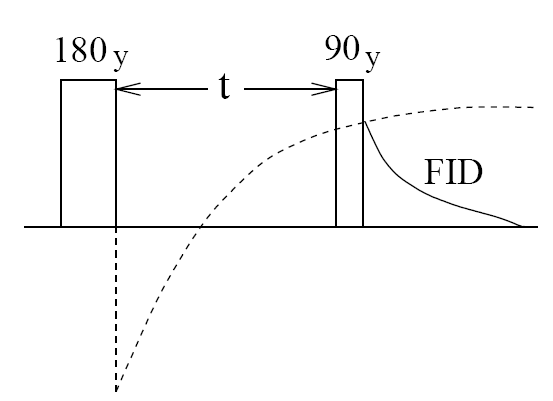
\includegraphics[width=0.5\textwidth]{images/T1_messung.png}
    \caption{Das Inversion Recovery-Experiment zur Messung der Spin-Gitter-Relaxationszeit $T_1$}
    \label{fig:T1_messung}
\end{figure}

\subsubsection{Messung von \texorpdfstring{$T_2$}{T2}}
\label{sssec:T2_Messung}

Zunächst soll das Hahn-Echo-Verfahren erklärt werden.
Dieses Verfahren nutzt die Reversibilität der Einflüsse der Feldinhomogenitäten um diese Einflüsse zu bereinigen und $T_2$ messen zu können.
Durch einen $\SI{90}{\degree}$-Puls wird der FID angeregt.
Durch einen $\SI{180}{\degree}$-Puls nach der Zeit $\tau$ werden alle Kernspin-Momente an der $y$-Achse gespiegelt. (siehe \autoref{fig:hahn_echo})
Die zuvor auseinanderlaufenden Spins laufen nun wieder aufeinander zu und so entsteht nach einer Zeit $2\tau$ ein Echo, das einen messbaren FID-Strom erzeugt.
Durch die Höhe des Echos kann die Spin-Spin-Relaxation 
\begin{equation}
    M_{x,y}(t) = M_{x,y}(t=0) \exp\left(-\frac{t}{T_2}\right)
\end{equation}
abgelesen werden. Wobei statt $t$ immer nur $2\tau$ betrachtet wird.

\begin{figure}
    \centering
    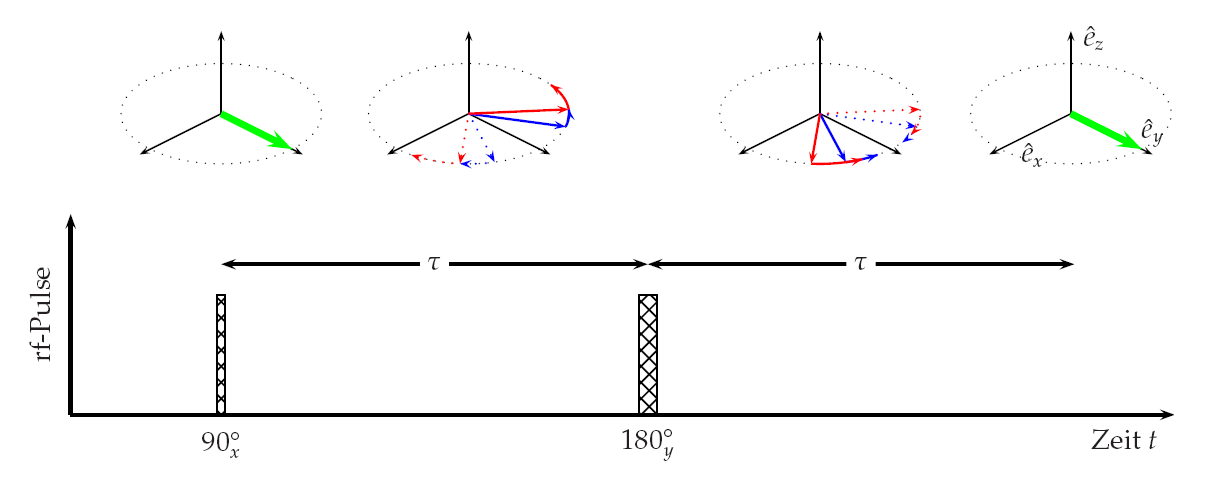
\includegraphics[width=\textwidth]{images/hahn_echo_2.png}
    \caption{Refokussierung der Magnetisierung durch ein Hahn-Echo \cite{V49}}
    \label{fig:hahn_echo}
\end{figure}

Damit nicht pro Messung nur ein Echo gemessen werden kann, wird die Hahn-Echo-Methode auf die Carr-Purcell-Methode erweitert
indem weitere $2\tau$-äquidistante $\SI{180}{\degree}$-Pulse ausgesendet werden 
und so weitere Refokussierungen und damit Echos zustande kommen.
Das Problem der Carr-Purcell-Methode ist, dass eine nicht exakte Länge des $\SI{180}{\degree}$-Pulses
dazu führt, dass die Magnetisierung nicht exakt in die $xy$-Ebene gedreht wird und so nach jedem Puls ein Fehler aufaddiert wird.

Dieses Problem wird gelöst mit der Meiboom-Gill-Methode, in der die $\SI{180}{\degree}$-Pulse um $\SI{90}{\degree}$ zu dem $\SI{90}{\degree}$-Puls ist.
So ist der Fehler in der Länge des $\SI{90}{\degree}$-Pulses egal und die Fehler der $\SI{180}{\degree}$-Pulse gleichen sich bei jedem zweiten Puls wieder aus.
Also ergibt sich hier für alle Echos bei $4n\tau$ die korrekte Amplitude und diese können verwendet werden um $T_2$ zu bestimmen.
\section{Durchführung}
\label{sec:Durchführung}


\section{Auswertung}
\label{sec:Auswertung}

Alle hier angegebenen Unsicherheiten wurden mit der Python Bibliothek Uncertainties berechnet.\cite{uncertainties}
Diese Bibliothek basiert auf der Gauß'schen Fehlerfortpflanzung
\begin{equation}
    \Delta y = \sum_{i=1}^n \left| \frac{\delta f(x_1,...,x_n)}{\delta x_i} \right| \Delta x_i \, .
    \label{eq:fehlerrechnung}
\end{equation}

Ziel dieser Auswertung ist es mit Hilfe der gepulsten Kernspinresonanz den Diffusionskoeffizienten $D$ zu berechnen. 
Damit diese Berechnung gelingt werden zunächst die beiden Relaxationszeiten $T_1$ und $T_2$ berechnet.
Als letzte Überprüfung der Auswertung wird der Molekülradius von Wasser über die gemessenen Werte bestimmt.

\subsection{Bestimmung von $T_1$}
\label{ssec:aus1}

Für die Berechnung von $T_1$ wird zunächst ein $\SI{180}{\degree}$-Puls durchgeführt.
Nach einer Zeitspanne $\tau$ folgt ein $\SI{90}{\degree}$-Puls. 
Die danach gemessenen Spannungen $U$ sind für verschiedene Werte $\tau$ in \autoref{tab:t1} notiert. 

\begin{table}
    \centering
    \caption{Gemessene Spannungen in Abhängigkeit von $\tau$ für die $T_1$ Bestimmung}
    \label{tab:t1}
    \begin{tabular}{S[table-format=5.1] S[table-format=4.0]}
        \toprule
        \tableSI{\tau}{\milli\second} & \tableSI{U}{\milli\volt}  \\
        \midrule
        1.0 &  -1075  \\
        1.6 & -1013 \\
        2.6 & -994 \\
        4.3 & -1000 \\
        7.0 & -1075 \\
        11.3 & -1037 \\
        18.3 & -1012 \\
        29.8 & -998 \\
        48.3 & -956 \\
        78.5 & -931 \\
        127.0 & -888 \\
        207.0 & -799 \\
        336.0 & -708 \\
        546.0 & -580 \\
        886.0 & -415 \\
        1440.0 & -201 \\
        2340.0 & 66 \\
        3000.0 & 117 \\
        3800.0 & 309 \\
        6160.0 & 508 \\
        10000.0 & 545 \\
        \bottomrule
    \end{tabular}
\end{table}

Anschließend werden diese Werte mit der Fit-Funktion 
\begin{equation}
    U(\tau) = a \cdot \exp(\frac{- \tau}{T_1}) + c 
    \label{eq:fit_t1}
\end{equation}
gefittet.
Dabei ergeben sich die Parameter 
\begin{align*}
    a =& \SI{-1.55(03)}{\volt} \\
    T_1 =& \SI{1.93(12)}{\second} \\
    c =& \SI{0.53(03)}{\volt} \, .
\end{align*}
Die Werte aus \autoref{tab:t1} sind in nachfolgend aufgetragen.
$T_1$ ist damit direkt aus dem Fit als 
\begin{equation*}
    T_1 = \SI{1.93(12)}{\second}
\end{equation*}
bestimmt worden.

\begin{figure}
    \centering
    \includegraphics[width=\textwidth]{build/plot_T1.pdf}
    \caption{Plot der Messwerte zur Messsung von $T_1$ mit exponentiellem Fit und logarithmischer X-Achse}
    \label{fig:t1}
\end{figure}

\subsection{Bestimmung von $T_2$}
\label{ssec:aus2}

Die vom Oszilloskop aufgenommenen Daten werden ebenfalls geplottet.
Allerdings sind hier nur die Maxima der Oszillazion für die Auswertung relevant.
Durch diese wird eine Fit-Funktion 
\begin{equation}
    U(\tau) = a \cdot \exp(\frac{- \tau}{T_2}) + c 
    \label{eq:fit_t2}
\end{equation}
gelegt.
Für diesen Fit werden die Parameter 
\begin{align*}
    a =& \SI{0.91(04)}{\per\volt} \\
    T_2 =& \SI{1.70(16)}{\second} \\
    c =& \SI{0.08(05)}{\volt} \, .
\end{align*}
bestimmt.
Die geplotteten Werte sind dann zusammen mit der Fit-Funktion in \autoref{fig:t2} dargestellt.
Auch hier die gesuchte Größe einer der gesuchen Parameter, sodass sich 
\begin{equation}
    T_2 = \SI{1.70(16)}{\second} 
    \label{eq:t2_wert}
\end{equation}
ergibt.
\begin{figure}
    \centering
    \includegraphics[width=\textwidth]{build/plot_T2.pdf}
    \caption{Plot der Messwerte zur Messsung von $T_2$ mit exponentiellem Fit}
    \label{fig:t2}
\end{figure}

Es wurden ebenfalls Oszilloskop-Daten genommen, bei denen die Einstellung "MG" auf "off" stand.
Das bedeutet, die Messung wurde nicht mit der Meiboom-Gill-Methode durchgeführt.
Dieser Plot ist nachfolgend in \autoref{fig:mgoff} aufgezeigt.
Eine Bestimmung von $T_2$ ist aus diesen Messdaten nicht möglich.

\begin{figure}
    \centering
    \includegraphics[width=\textwidth]{build/plot_mgoff.pdf}
    \caption{Messdaten des Oszilloskops ohne Meiboom-Gill-Methode}
    \label{fig:mgoff}
\end{figure}

\subsection{Bestimmung des Diffusionskoeffizienten $D$}
\label{ssec:aus3}

Zur erfolgreichen Berechung von $D$ über GLEICHUNG VON NICO werden die Gradiantenstärke $G$ und die Zeitkonstante $T_\text{D}$ benötigt. 
Diese beiden Größen werden im Folgenden bestimmt.

Für die Berechnung der Gradiantenstärke $G$ wird das Oszillatorbild des Echos zunächst in \autoref{fig:echo} dargestellt.
Die eigentliche Bestimmung kann aber erst nach einer Fouriertransformation stattfinden. 
Alle Werte vor dem Maximum des Realteils werden hierbei verworfen.
Die Fouriertransformierte ist \autoref{fig:fourier} stark vergrößert, da der Durchmesser $d_\text{f}$ des entstandenen Halbkreises benötigt wird.

\begin{figure}
    \centering
    \begin{subfigure}{0.4\textwidth}
        \centering
        \includegraphics[width=\textwidth]{build/plot_Diff.pdf}
        \caption{Echo bei $\tau = \SI{0.2}{\milli\second}$}
        \label{fig:echo}
    \end{subfigure}
    \begin{subfigure}{0.4\textwidth}
        \centering
        \includegraphics[width=\textwidth]{build/plot_echo_Gradient.pdf}
        \caption{Stark vergrößerte Fouriertransformation des Echos}
        \label{fig:fourier}
    \end{subfigure}
    \caption{Aufgenommenes Echo mit entsprechender Fouriertransformation zur Bestimmung der Gradiantenstärke}
    \label{fig:g_messung}
\end{figure}

Der Durchmesser des Halbkreises wird etwa als 
\begin{equation*}
    d_\text{f} = \SI{13300}{\hertz} 
    \label{eq:df}
\end{equation*}
abgelesen.
Über FORMEL AUS THEORIE kann dann $G$ 
\begin{equation}
    G = \frac{2 \pi \cdot d_\text{f}}{\gamma _\text{H} \cdot d} = \SI{0.071}{\tesla\per\meter}
    \label{eq:g_wert}
\end{equation}
berechnet werden.
Dabei sind
\begin{align*}
    \gamma _\text{H} =& \, \SI{268e6}{\radian\per\second\per\tesla} \\
    d =& \, \SI{4.4}{\milli\meter} \, . 
\end{align*}
$\gamma _\text{H}$ ist das gyromagnetische Verhältnis von Protonen in Wasser. \cite{physics_constants}

$T_\text{D}$ erhalten wir aus einem exponentiellen Fit durch die Messwerte in \autoref{tab:diff}.
Hierbei ist wichtig anzumerken, dass es im Intervall $\SI{0.1}{\second}$ bis $\SI{1}{\second}$ noch weitere Werte gab.
Diese lagen allerdings sehr dicht aneinander und haben den Fit teilweise verfälscht.

\begin{table}
    \centering
    \caption{Gemessene Spannungen in Abhängigkeit von $\tau$ für die Bestimmung des Diffusionskoeffizienten}
    \label{tab:diff}
    \begin{tabular}{S[table-format=2.1] S[table-format=4.0]}
        \toprule
        \tableSI{\tau}{\milli\second} & \tableSI{U}{\milli\volt}  \\
        \midrule
        0.3 & 1275 \\
        1.0 & 1258 \\
        2.0 & 1260 \\
        4.0 & 1213 \\
        6.0 & 1103 \\
        8.0 & 925 \\
        10.0 & 698 \\
        10.0 & 639 \\
        11.0 & 571 \\
        12.0 & 461 \\
        13.0 & 356 \\
        14.0 & 257 \\
        15.0 & 194 \\
        16.0 & 127 \\
        17.0 & 93 \\
        18.0 & 65 \\
        19.0 & 50 \\
        20.0 & 46 \\
        \bottomrule
    \end{tabular}
\end{table}

Der Fit wird dabei mit der Funktion 
\begin{equation}
    U(\tau) = a \cdot \exp(\frac{- 2\,  \tau}{T_2}) \, \exp(- \tau ^3 \cdot 2 \, b) + c 
    \label{eq:fit_d}
\end{equation}
durchgeführt.
Hierbei ist $T_2$ der oben berechnete Wert.
Die Parameter, die sich dabei ergeben sind 
\begin{align*}
    a =& \SI{1.236(3)}{\per\volt} \\
    b =& \SI{304556.538(2050836)}{\per\cubic\second} \\
    c =& \SI{0.033(2)}{\volt} \, .
\end{align*}
Es ergibt sich der Plot in \autoref{fig:diff}, wobei der Fit in Basiseinheiten durchgeführt wurde.
\begin{figure}
    \centering
    \includegraphics[width=\textwidth]{build/plot_Diff3.pdf}
    \caption{Plot der Messwerte zur Messsung von $D$ mit exponentiellem Fit}
    \label{fig:diff}
\end{figure}

Wird nun die Fit-Funktion mit THEORIEFORMEL verglichen, ergibt sich der folgende Zusammenhang,
\begin{equation}
    T_\text{D} = \frac{2 \, b}{\tau ^2} \, . 
    \label{eq:b_td}
\end{equation}
Damit ist es nun möglich über THEORIEFORMEL den Diffusionskoeffizienten $D$ zu berechnen.
Die Gradientenstärke $G$ haben wir bereits bestimmt und $\gamma _\text{H}$ ist das bekannte gyromagnetische Verhältnis von Protonen.
Wir erhalten die Formel 
\begin{equation}
    D = \frac{3 \, b}{\gamma _\text{H}^2 \, G^2 } \, . 
    \label{eq:diffusion}
\end{equation}
Und so ergibt sich 
\begin{equation*}
    D = \SI{2.533(17)e-9}{\meter\squared\per\second} \, . 
    \label{eq:diffusion_wert}
\end{equation*}

\subsection{Abschließende Berechnung des Molekülradius}
\label{ssec:aus4}

Der Molekülradius von Wasser wird über die Einstein-Stokes-Formel berechnet.
Formt man THEORIEFORMEL nach dem Radius $r$ um, ergibt sich 
\begin{equation}
    r =  \frac{K_\text{B} \, T}{6 \, \pi \, \eta \, D } \, .
    \label{eq:stokes}
\end{equation}
$\eta$ ist die Viskosität von Wasser $\eta = \SI{1}{\milli\pascal\second} $ und $K_\text{B}$ die Boltzmann-Konstante. \cite{wasser}
Die Temperatur $T$ wurde vor und nach dem Versuch gemessen, diese sind 
\begin{align*}
    T_\text{vor} =& \SI{295.25}{\kelvin} \\
    T_\text{nach} =& \SI{296.45}{\kelvin} \, .
\end{align*}
Da die Bestimmung von $D$ gegen Ende des Versuches stattfand, wird hier $T_\text{nach}$ verwendet.
Dadurch ergibt sich dann für den Molekülradius von Wasser
\begin{equation*}
    r_\text{mess} = \SI{0.857(6)}{\angstrom}  \, .
    \label{eq:radius1}
\end{equation*}

Den Vergleichswert berechnen wir über
\begin{equation}
    r =  \sqrt[3]{ \left(  \frac{M_\text{W}}{\frac{4}{3} \, \pi \, \rho \, N_\text{A} }  \right)} \, .
    \label{eq:hexagonal}
\end{equation}
Die benötigten Konstanten sind die Molekulardichte von Wasser $\rho _\text{W} = \SI{1}{\gram\per\cubic\centi\meter}$ und die Molmasse von Wasser
$M _\text{W} = \SI{18.015}{\gram\per\mol}$. \cite{wasser}
$N_\text{A}$ ist die Avogadro-Konstante.
Der Theoriewert ist dann 
\begin{equation*}
    r_\text{theorie} = \SI{1.742}{\angstrom}  \, .
    \label{eq:radius2}
\end{equation*}

\section{Diskussion}
\label{sec:Diskussion}

\subsection{Vergleich von \texorpdfstring{$T_1$}{T1}}

Zunächst wird der von uns berechnete Wert für die Spin‐Gitter‐Relaxationszeit $T_1$ mit dem Literaturwert $T_{1,\text{lit}}$ verglichen. \cite{T1}
Die Werte sind dabei 
\begin{align*}
    T_1 &= \SI{1.93(12)}{\second} \\
    T_{1,\text{lit}} &= \SI{3.15}{\second} \, .
\end{align*}
Der Literaturwert entspricht der Relaxationszeit bei einer Temperatur von $T = \SI{20}{\celsius}$, da zu Beginn des Versuches die Temperatur 
$T = \SI{22.1}{\celsius}$ betrug.
Die Abweichung von einander ist somit
\begin{equation}
    \Delta T_1 = \num{34.92} \% \, .
\end{equation}
Das ist eine relativ hohe Abweichung.
Betrachtet man \autoref{fig:t1}, den Plot der zur Auswertung verwendet wurde, wird auch teilweise klar warum.
Zu Beginn liegen einige der Messwerte nicht wirklich auf der Fit-Funktion.
Das liegt vor allem daran, dass die Messwerte kurzzeitig sinken, obwohl das eigentlich nicht passieren dürfte.
Es ist davon auszugehen, dass hier etwas nicht korrekt funktioniert hat. 
Diese Werte wurden von einem Oszilloskop abgelesen, weswegen ein systematischer Fehler aufgetreten sein könnte.

\subsection{Diffusionskoeffizient und Molekülradius}

Der Diffusionskoeffizient wird ebenfalls mit einem Literaturwert vergleichen. 
Da diese Messung gegen Ende stattfand, wird hier der Wert für $T = \SI{25}{\celsius}$ verwendet. \cite{D}
Die Messwerte für $D$ sind dann
\begin{align*}
    D &= \SI{2.533(17)e-9}{\meter\squared\per\second} \\
    D_\text{lit} &= \SI{2.299e-9}{\meter\squared\per\second} \, .
\end{align*}
Damit erhalten wir eine Abweichung von 
\begin{equation}
    \Delta D = \num{8.62} \% \, .
\end{equation}
Vergleichen mit der vorherigen Abweichung erscheint diese wesentlich genauer zu sein. 
Das liegt aber auch vor allem daran, dass wir einige sehr schlechte Werte entfernt haben, wie bereits erwähnt. 
So konnten die Parameter des Fits sehr genau bestimmt werden.

Die letzte Überprüfung der Genauigkeit dieser Messung findet bei der Bestimmung der Molekülradien statt.
Beide möglichen Werte wurden bereits in der Auswertung bestimmt. 
Daher wird hier nur die Abweichung 
\begin{equation}
    \Delta r = \num{50.46} \% \, .
\end{equation}
berechnet.
Die Abweichung ist offensichtlich recht groß.
Einerseits war $D$ natürlich eine fehlerbehaftete Größe und somit nicht exakt bestimmt.
Zudem wurde hier eine Temperatur angegeben, die erst nach der eigentlichen Messung bestimmt worden war.
Vor allem war die Viskosität $\eta$ aber nicht exakt an die Temperatur angepasst. 
Die Viskosität ändert sich mit der Temperatur und wir konnten die Viskositätsmessung nicht durchführen.

\printbibliography{}

% Python Code Anhang
\section*{Anhang: Python Code der Auswertung der Messung}
\addcontentsline{toc}{section}{Anhang}

\inputminted[linenos,breaklines]{python}{python/messung.py}

\end{document}
